% This file was converted to LaTeX by Writer2LaTeX ver. 1.4
% see http://writer2latex.sourceforge.net for more info
\documentclass[12pt]{article}
\usepackage[utf8]{inputenc}
\usepackage[T1]{fontenc}
\usepackage[english]{babel}
\usepackage{amsmath}
\usepackage{amssymb,amsfonts,textcomp}
\usepackage{array}
\usepackage{supertabular}
\usepackage{hhline}
\usepackage{hyperref}
\hypersetup{colorlinks=true, linkcolor=blue, citecolor=blue, filecolor=blue, urlcolor=blue}
\usepackage{graphicx}
% footnotes configuration
\makeatletter
\renewcommand\thefootnote{\arabic{footnote}}
\makeatother
% Text styles
\newcommand\textstyleListLabelxix[1]{#1}
\makeatletter
\newcommand\arraybslash{\let\\\@arraycr}
\makeatother
\raggedbottom
% Paragraph styles
\renewcommand\familydefault{\rmdefault}
\newenvironment{styleStandard}{\setlength\leftskip{0cm}\setlength\rightskip{0cm plus 1fil}\setlength\parindent{0cm}\setlength\parfillskip{0pt plus 1fil}\setlength\parskip{0in plus 1pt}\writerlistparindent\writerlistleftskip\leavevmode\normalfont\normalsize\writerlistlabel\ignorespaces}{\unskip\vspace{0.111in plus 0.0111in}\par}
\newenvironment{stylelsSectioni}{\setlength\leftskip{0.25in}\setlength\rightskip{0in plus 1fil}\setlength\parindent{0in}\setlength\parfillskip{0pt plus 1fil}\setlength\parskip{0.1665in plus 0.016649999in}\writerlistparindent\writerlistleftskip\leavevmode\normalfont\normalsize\fontsize{18pt}{21.6pt}\selectfont\bfseries\writerlistlabel\ignorespaces}{\unskip\vspace{0.0835in plus 0.00835in}\par}
\newenvironment{stylelsSectionii}{\setlength\leftskip{0.25in}\setlength\rightskip{0in plus 1fil}\setlength\parindent{0in}\setlength\parfillskip{0pt plus 1fil}\setlength\parskip{0.222in plus 0.0222in}\writerlistparindent\writerlistleftskip\leavevmode\normalfont\normalsize\fontsize{16pt}{19.2pt}\selectfont\bfseries\writerlistlabel\ignorespaces}{\unskip\vspace{0.0835in plus 0.00835in}\par}
\newenvironment{styleListParagraph}{\setlength\leftskip{0.5in}\setlength\rightskip{0in plus 1fil}\setlength\parindent{0in}\setlength\parfillskip{0pt plus 1fil}\setlength\parskip{0in plus 1pt}\writerlistparindent\writerlistleftskip\leavevmode\normalfont\normalsize\writerlistlabel\ignorespaces}{\unskip\vspace{0.111in plus 0.0111in}\par}
\newenvironment{styleQuote}{\setlength\leftskip{0.3937in}\setlength\rightskip{0.3937in plus 1fil}\setlength\parindent{0in}\setlength\parfillskip{0pt plus 1fil}\setlength\parskip{0in plus 1pt}\writerlistparindent\writerlistleftskip\leavevmode\normalfont\normalsize\writerlistlabel\ignorespaces}{\unskip\vspace{0.1965in plus 0.019650001in}\par}
\newenvironment{stylelsAbstract}{\setlength\leftskip{0.5in}\setlength\rightskip{0.5in}\setlength\parindent{0in}\setlength\parfillskip{0pt plus 1fil}\setlength\parskip{0in plus 1pt}\writerlistparindent\writerlistleftskip\leavevmode\normalfont\normalsize\itshape\writerlistlabel\ignorespaces}{\unskip\vspace{0.111in plus 0.0111in}\par}
% List styles
\newcommand\writerlistleftskip{}
\newcommand\writerlistparindent{}
\newcommand\writerlistlabel{}
\newcommand\writerlistremovelabel{\aftergroup\let\aftergroup\writerlistparindent\aftergroup\relax\aftergroup\let\aftergroup\writerlistlabel\aftergroup\relax}
\newcounter{listWWNumxxiileveli}
\newcounter{listWWNumxxiilevelii}[listWWNumxxiileveli]
\newcounter{listWWNumxxiileveliii}[listWWNumxxiilevelii]
\newcounter{listWWNumxxiileveliv}[listWWNumxxiileveliii]
\renewcommand\thelistWWNumxxiileveli{\arabic{listWWNumxxiileveli}}
\renewcommand\thelistWWNumxxiilevelii{\arabic{listWWNumxxiileveli}.\arabic{listWWNumxxiilevelii}}
\renewcommand\thelistWWNumxxiileveliii{\arabic{listWWNumxxiileveli}.\arabic{listWWNumxxiilevelii}.\arabic{listWWNumxxiileveliii}}
\renewcommand\thelistWWNumxxiileveliv{\arabic{listWWNumxxiileveli}.\arabic{listWWNumxxiilevelii}.\arabic{listWWNumxxiileveliii}.\arabic{listWWNumxxiileveliv}}
\newcommand\labellistWWNumxxiileveli{\thelistWWNumxxiileveli.}
\newcommand\labellistWWNumxxiilevelii{\thelistWWNumxxiilevelii.}
\newcommand\labellistWWNumxxiileveliii{\thelistWWNumxxiileveliii.}
\newcommand\labellistWWNumxxiileveliv{\thelistWWNumxxiileveliv.}
\newenvironment{listWWNumxxiileveli}{\def\writerlistleftskip{\setlength\leftskip{0.5in}}\def\writerlistparindent{}\def\writerlistlabel{}\def\item{\def\writerlistparindent{\setlength\parindent{-0.25in}}\def\writerlistlabel{\stepcounter{listWWNumxxiileveli}\makebox[0cm][l]{\labellistWWNumxxiileveli}\hspace{-0.635cm}\writerlistremovelabel}}}{}
\newenvironment{listWWNumxxiilevelii}{\def\writerlistleftskip{\setlength\leftskip{1in}}\def\writerlistparindent{}\def\writerlistlabel{}\def\item{\def\writerlistparindent{\setlength\parindent{-0.25in}}\def\writerlistlabel{\stepcounter{listWWNumxxiilevelii}\makebox[0cm][l]{\labellistWWNumxxiilevelii}\hspace{-1.905cm}\writerlistremovelabel}}}{}
\newenvironment{listWWNumxxiileveliii}{\def\writerlistleftskip{\setlength\leftskip{1.5in}}\def\writerlistparindent{}\def\writerlistlabel{}\def\item{\def\writerlistparindent{\setlength\parindent{-0.1252in}}\def\writerlistlabel{\stepcounter{listWWNumxxiileveliii}\makebox[0cm][r]{\labellistWWNumxxiileveliii}\hspace{-3.4919918cm}\writerlistremovelabel}}}{}
\newenvironment{listWWNumxxiileveliv}{\def\writerlistleftskip{\setlength\leftskip{2in}}\def\writerlistparindent{}\def\writerlistlabel{}\def\item{\def\writerlistparindent{\setlength\parindent{-0.25in}}\def\writerlistlabel{\stepcounter{listWWNumxxiileveliv}\makebox[0cm][l]{\labellistWWNumxxiileveliv}\hspace{-4.4449997cm}\writerlistremovelabel}}}{}
\newcounter{listWWNumxxiiileveli}
\newcounter{listWWNumxxiiilevelii}[listWWNumxxiiileveli]
\newcounter{listWWNumxxiiileveliii}[listWWNumxxiiilevelii]
\newcounter{listWWNumxxiiileveliv}[listWWNumxxiiileveliii]
\renewcommand\thelistWWNumxxiiileveli{\arabic{listWWNumxxiiileveli}}
\renewcommand\thelistWWNumxxiiilevelii{\alph{listWWNumxxiiilevelii}}
\renewcommand\thelistWWNumxxiiileveliii{\roman{listWWNumxxiiileveliii}}
\renewcommand\thelistWWNumxxiiileveliv{\arabic{listWWNumxxiiileveliv}}
\newcommand\labellistWWNumxxiiileveli{(\thelistWWNumxxiiileveli)}
\newcommand\labellistWWNumxxiiilevelii{\thelistWWNumxxiiilevelii.}
\newcommand\labellistWWNumxxiiileveliii{\thelistWWNumxxiiileveliii.}
\newcommand\labellistWWNumxxiiileveliv{\thelistWWNumxxiiileveliv.}
\newenvironment{listWWNumxxiiileveli}{\def\writerlistleftskip{\setlength\leftskip{0.75in}}\def\writerlistparindent{}\def\writerlistlabel{}\def\item{\def\writerlistparindent{\setlength\parindent{-0.25in}}\def\writerlistlabel{\stepcounter{listWWNumxxiiileveli}\makebox[0cm][l]{\labellistWWNumxxiiileveli}\hspace{-1.27cm}\writerlistremovelabel}}}{}
\newenvironment{listWWNumxxiiilevelii}{\def\writerlistleftskip{\setlength\leftskip{1.25in}}\def\writerlistparindent{}\def\writerlistlabel{}\def\item{\def\writerlistparindent{\setlength\parindent{-0.25in}}\def\writerlistlabel{\stepcounter{listWWNumxxiiilevelii}\makebox[0cm][l]{\labellistWWNumxxiiilevelii}\hspace{-2.54cm}\writerlistremovelabel}}}{}
\newenvironment{listWWNumxxiiileveliii}{\def\writerlistleftskip{\setlength\leftskip{1.75in}}\def\writerlistparindent{}\def\writerlistlabel{}\def\item{\def\writerlistparindent{\setlength\parindent{-0.1252in}}\def\writerlistlabel{\stepcounter{listWWNumxxiiileveliii}\makebox[0cm][r]{\labellistWWNumxxiiileveliii}\hspace{-4.1269917cm}\writerlistremovelabel}}}{}
\newenvironment{listWWNumxxiiileveliv}{\def\writerlistleftskip{\setlength\leftskip{2.25in}}\def\writerlistparindent{}\def\writerlistlabel{}\def\item{\def\writerlistparindent{\setlength\parindent{-0.25in}}\def\writerlistlabel{\stepcounter{listWWNumxxiiileveliv}\makebox[0cm][l]{\labellistWWNumxxiiileveliv}\hspace{-5.08cm}\writerlistremovelabel}}}{}
\newcommand\labellistWWNumxxivleveli{[F0B7?]}
\newcommand\labellistWWNumxxivlevelii{\textstyleListLabelxix{o}}
\newcommand\labellistWWNumxxivleveliii{[F0A7?]}
\newcommand\labellistWWNumxxivleveliv{[F0B7?]}
\newenvironment{listWWNumxxivleveli}{\def\writerlistleftskip{\setlength\leftskip{0.5in}}\def\writerlistparindent{}\def\writerlistlabel{}\def\item{\def\writerlistparindent{\setlength\parindent{-0.25in}}\def\writerlistlabel{\makebox[0cm][l]{\labellistWWNumxxivleveli}\hspace{-0.635cm}\writerlistremovelabel}}}{}
\newenvironment{listWWNumxxivlevelii}{\def\writerlistleftskip{\setlength\leftskip{1in}}\def\writerlistparindent{}\def\writerlistlabel{}\def\item{\def\writerlistparindent{\setlength\parindent{-0.25in}}\def\writerlistlabel{\makebox[0cm][l]{\labellistWWNumxxivlevelii}\hspace{-1.905cm}\writerlistremovelabel}}}{}
\newenvironment{listWWNumxxivleveliii}{\def\writerlistleftskip{\setlength\leftskip{1.5in}}\def\writerlistparindent{}\def\writerlistlabel{}\def\item{\def\writerlistparindent{\setlength\parindent{-0.25in}}\def\writerlistlabel{\makebox[0cm][l]{\labellistWWNumxxivleveliii}\hspace{-3.175cm}\writerlistremovelabel}}}{}
\newenvironment{listWWNumxxivleveliv}{\def\writerlistleftskip{\setlength\leftskip{2in}}\def\writerlistparindent{}\def\writerlistlabel{}\def\item{\def\writerlistparindent{\setlength\parindent{-0.25in}}\def\writerlistlabel{\makebox[0cm][l]{\labellistWWNumxxivleveliv}\hspace{-4.4449997cm}\writerlistremovelabel}}}{}
\setlength\tabcolsep{1mm}
\renewcommand\arraystretch{1.3}
\title{}
\author{Lukasz Grabowski}
\date{2020-09-16}
\begin{document}
\clearpage\setcounter{page}{1}\begin{styleStandard}
\textbf{\textsuperscript{Grammar patterns as an exploratory tool for studying formulaicity in English-to-Polish translation: a corpus-based study }}
\end{styleStandard}

\begin{styleStandard}
Łukasz Grabowski\textsuperscript{1}, Nicholas Groom\textsuperscript{2}
\end{styleStandard}

\begin{styleStandard}
\textsuperscript{1}University of Opole, \textsuperscript{2}University of Birmingham
\end{styleStandard}

\begin{styleStandard}
\textbf{Abstract.} In this chapter, we explore the use – and argue for the usefulness – of the concept of grammar patterns (Francis et al 19966, 1998; Hunston \& Francis 1999) in descriptive research on the English-to-Polish translation of formulaic language. Specifically, we use the \textit{Paralela} English-Polish parallel corpus (Pęzik 2016) to explore – largely in terms of frequency distributions – the use of the Polish equivalents of selected English multi-word items, which are textual manifestations of grammar patterns. As a proof-of-concept, we will focus on a pre-selected grammar pattern (‘\textit{it} v-link ADJ \textit{to}{}-inf’), where a given word (e.g. the adjective \textit{possible}) may convey different senses depending on the pattern in which it occurs (Groom 2005). We aim to check whether and to what extent somewhat similar lexico-grammatical patterns emerge from the Polish language data (i.e. from the Polish translations under scrutiny). Using this method, we are also able to investigate whether the Polish equivalents of that English grammar pattern (i.e. from its textual manifestations) are realized with the same level of regularity in translation. Early findings revealed the English pattern ‘\textit{it} v-link ADJ \textit{to}{}-inf’, when filled by adjectives conveying the sense of ‘difficulty’, corresponds to a set of Polish syntagmatic patterns, such as ‘ADJ v-link, \textit{aby}’, ‘ADV v-link’ or ‘ADV’ (the last two ones followed by verbs in the infinitive form), which contribute to the formulaicity of Polish texts. It is argued not only that the study’s findings indicate that grammar patterns are a useful starting point for the exploration of formulaicity in translation, but also that they help us explain some more general differences in terms of semantics, pragmatics and usage in source texts and their translations.
\end{styleStandard}


\setcounter{listWWNumxxiileveli}{0}
\begin{listWWNumxxiileveli}
\item 
\begin{stylelsSectioni}
Introduction.
\end{stylelsSectioni}


\setcounter{listWWNumxxiilevelii}{0}
\begin{listWWNumxxiilevelii}
\item 
\begin{stylelsSectionii}
General remarks on Pattern Grammar
\end{stylelsSectionii}
\end{listWWNumxxiilevelii}
\end{listWWNumxxiileveli}
\begin{styleStandard}
In the last three decades, corpus linguists have proposed a number of novel research methods and procedures for capturing and exploring recurrent patterns of language use. One of them is Pattern Grammar (Hunston \& Francis 2000), a corpus-based grammar of the English language that describes the lexico-syntactic environments of individual lexical items. These ‘grammar patterns’ (henceforth GPs) are defined as “a phraseology frequently associated with (a sense of) a word, particularly in terms of the prepositions, groups, and clauses that follow the word” (Hunston \& Francis 2000: 3) or as “all the words and structures which are regularly associated with the word and which contribute to its meaning” (ibid. 37). As argued by Roemer (2009: 142), GPs are neither single words nor empty grammatical structures; they constitute abstract representations of frequent lexico-grammatical patterns. For example, Hunston and Francis (2000: 29) claim that in the patterns \textbf{\textit{it }}\textbf{v-link ADJ that} (e.g. \textit{it is interesting/clear that}) \textit{\ }and \textbf{\textit{it }}\textbf{v-link ADJ }\textbf{\textit{to}}\textbf{{}-inf} (e.g. \textit{it is sensible/possible to}), the adjectives belong to similar meaningfully-related groups, e.g. expressing a range of different concepts such as likelihood, importance, desirability and obviousness. 
\end{styleStandard}

\begin{styleStandard}
Whilst Pattern Grammar is principally an empirical approach to linguistic description, it also puts forward two major theoretical claims. The first of these is that the different meanings (i.e. senses) of polysemous words can be distinguished on the basis of their typical occurrence in different patterns. Consider, by way of example, the following two (invented) sentences: 
\end{styleStandard}


\setcounter{listWWNumxxiiileveli}{0}
\begin{listWWNumxxiiileveli}
\item 
\begin{styleStandard}
\textbf{\textit{It’s possible that}}\textit{ she sent a message.}
\end{styleStandard}
\item 
\begin{styleStandard}
\textbf{\textit{It’s possible to}}\textit{ send a message.}
\end{styleStandard}
\end{listWWNumxxiiileveli}
\begin{styleStandard}
It should be immediately clear that, although the GPs highlighted in bold in these sentences both feature the same adjective, \textbf{\textit{possible}}, the meanings that they make are very different. In example (1), the highlighted words can be replaced with the single adverb \textbf{\textit{maybe}}, whereas in example (2) the highlighted part can be replaced with the two words \textbf{\textit{you can}}. From a traditional perspective, it might be said that this shows that the adjective \textbf{\textit{possible}} has two different meanings: an epistemic modal meaning in example (1), and a dynamic modal meaning in example (2). From the point of view of Pattern Grammar, however, the epistemic and dynamic modal meanings made by these two sentences reside not in any of the individual words, nor in the morphosyntactic configurations into which these words fall, but in the interaction between them. That is, the epistemic ‘maybe’ meaning belongs to the whole sequence ‘\textit{it is} \textit{possible} + that-clause’, and the dynamic ‘you can’ meaning is made by the whole sequence ‘\textit{it is} \textit{possible} + to-infinitive clause’. This insight is of major significance because, if it is true for a language as a whole, it means that semantic ambiguity is virtually non-existent in naturally-occurring language. Each of the different meanings of a polysemous word will be associated with a different structural pattern, and language users will interpret which meaning is being made in each case on the basis of this patterning. In other words, Pattern Grammar proposes that disambiguation is far more a matter of attending to linguistic co-text than it is a matter of attending to extralinguistic context, as is generally assumed in traditional theories of semantics and pragmatics.
\end{styleStandard}

\begin{styleStandard}
The second major theoretical claim put forward by Pattern Grammar is that “words which share a given pattern tend also to share an aspect of meaning” (Hunston \& Francis 2000: 3). To return to examples (1) and (2) above, \textbf{\textit{possible}} is just one member of a class of adjectives that have a broadly epistemic modal meaning when they occur in the pattern \textbf{\textit{it}}\textbf{ v-link ADJ }\textbf{\textit{that}} (e.g. \textit{certain, definite, demonstrable, doubtful, feasible, implausible, incredible, irrefutable, likely, true, uncertain, unthinkable,} etc.), and just one of many adjectives that have a broadly dynamic modal meaning when they occur in the pattern \textbf{\textit{it}}\textbf{ v-link ADJ }\textbf{\textit{to}}\textbf{{}-inf }(e.g. \textit{difficult, easy, feasible, hard, impossible, impractical., simple, tough, tricky}, etc.). In Pattern Grammar, these classes of words that share a particular pattern/meaning association are referred to as ‘meaning groups’. It is important to note that each grammatical pattern is not restricted to just one meaning group; on the contrary, many if not most patterns have several different meaning groups associated with them. For example, Francis et al (1998) identify eight distinct meaning groups for the pattern \textbf{\textit{it}}\textbf{ v-link ADJ }\textbf{\textit{that}}, and nine different meaning groups for the pattern \textbf{\textit{it}}\textbf{ v-link ADJ to-}\textbf{\textit{inf}}. 
\end{styleStandard}

\begin{styleStandard}
Although Pattern Grammar is unquestionably a corpus-based approach to grammatical description, it is nevertheless highly reliant on the manual qualitative analysis of concordance lines, and thus on the application of human judgement in the identifying of patterns and the meaning groups associated with them. This is because the identification of GPs in attested language corpora essentially involves perceiving a similarity between linguistic items which may not be identical on the surface, but which have some underlying regularity of form and meaning, which at the current time can only be reliably identified by a human analyst.\footnote{The automatic identification of GPs has been demonstrated as feasible in principle (Mason \& Hunston 2004), \textrm{but has not as yet been achieved at scale on open text.}} For example, the sequence of words \textit{it is ironic that} is a representative of a general pattern beginning with it, ending with a \textit{that}{}-clause (with optional \textit{that}) and containing a linking verb (e.g. \textit{be, seem, look}), followed by an adjective expressing evaluation of a given situation, e.g. \textit{it is not surprising that, it looks very unlikely that, it seems very peculiar that} (Hunston \& Francis 2000: 154). Such judgements are often highly nuanced and subtle, and it is sometimes problematic even for human researchers, let alone computer software, to distinguish between sequences of words which are formally the same yet differ in terms of their patterns, e.g. ‘annoyance + relative clause’ vs. ‘annoyance + appositive that-clause’ (Hunston \& Francis 2000: 67). 
\end{styleStandard}

\begin{styleStandard}
Despite its labour intensive nature, Pattern Grammar has been widely and successfully applied to the description and analysis of English over the last two decades or so. Perhaps the best known fruits of this research are the two monumental \textit{COBUILD Grammar Patterns} reference works (Francis et al. 1996, 1998), one covering 700 patterns across 9,000 different verb senses, and the other covering 100 further patterns across 10,000 nouns and adjectives. In addition to these general reference works, corpus-based studies have also provided empirical evidence that GPs differ in systematic ways across different discourses and genres, with academic English being a particular focus of interest (e.g. Groom 2005; Charles 2006, 2007; Larsson 2016; Su \& Hunston 2019). The COBUILD Grammar Patterns reference works have also been used as an empirical basis for psycholinguistic investigations into first and second language speaker knowledge of verb argument constructions (e.g. Ellis et al. 2014; R\"{o}mer et al. 2014, 2015).
\end{styleStandard}

\begin{styleStandard}
These latter inter-varietal research perspectives suggest that Pattern Grammar might also be used to carry out empirical research in cross-linguistic contexts. Surprisingly, however, no work along such lines has been done to date; in fact, although there is some comparative cross-linguistic research on grammar patterns in the specialized genre of judicial decisions (Pontrandolfo \& Gozdz-Roszkowski 2014) focusing on the discoursal function of evaluation in English and Italian, PG has as yet never been systematically applied to any other language than English (Hunston, personal communication).
\end{styleStandard}


\setcounter{listWWNumxxiileveli}{0}
\begin{listWWNumxxiileveli}
\item 

\setcounter{listWWNumxxiilevelii}{0}
\begin{listWWNumxxiilevelii}
\item 
\begin{stylelsSectionii}
Towards Pattern Grammar for languages other than English
\end{stylelsSectionii}
\end{listWWNumxxiilevelii}
\end{listWWNumxxiileveli}
\begin{styleStandard}
In fact, there has been no usage-based description similar to Pattern Grammar capturing recurrent lexico-grammatical patterns of language use in Polish, i.e. based on the relationship between meanings or discourse functions on the one hand and structural patterns on the other. However, similar to valency dictionaries developed for English (e.g. \textit{Erlangen Valency Patternbank}\footnote{\textrm{EVP is available at: }\url{http://www.patternbank.uni-erlangen.de/cgi-bin/patternbank.cgi}\textrm{; it provides a list of valency patterns for 511 verbs, 544 adjectives and 274 nouns. See Herbst et al. (2004) for more details.}} or \textit{Pattern Dictionary of English Verbs}\footnote{\textrm{PDEV is available at: }\url{http://pdev.org.uk/\#about_cpa}\textrm{; it provides systematic description of meaning and use of verb patterns of 1451 verbs (as of 9 July 2019). See Hanks (2008a, 2013) for more details.}}), there are dictionaries of Polish that combine syntactic and semantic information on particular lexical items in ways which bear some comparison with the Pattern Grammar approach. One of them is \textit{Walenty}\footnote{ Primarily a dictionary of Polish subcategorization frames, Walenty can be directly compared to FrameNet (http://framenet. icsi.berkeley.edu) grounded in the theory of frame semantics (Fillmore 1982).}\textit{,} a comprehensive valency dictionary of Polish (Przepiórkowski et al. 2017a, 2017b) that specifies arguments of predicates for verbs (and – to a lesser extent – for nouns, adjectives and adverbs), which consist of comprehensive syntactic and semantic formalisms, the latter ones not fully implemented yet (Przepiórkowski et al. 2017a: 10). Although utilized by two parsers of Polish (\textit{Świgra} and POLFIE), the dictionary has been designed primarily for computer processing of natural language texts as well as for researchers (linguists) and lexicographers (ibid.: 9). For example (and unlike in the case of Pattern Grammar), verbs recorded in \textit{Walenty} are described using the valency frames, each with a set of argument specifications (ibid.), e.g. the verb \textit{otruć }(‘to poison’) has three syntactic frames and one semantic frame, all accompanied by examples of use (Figure 1).
\end{styleStandard}

\begin{styleStandard}
\   [Warning: Image ignored] % Unhandled or unsupported graphics:
%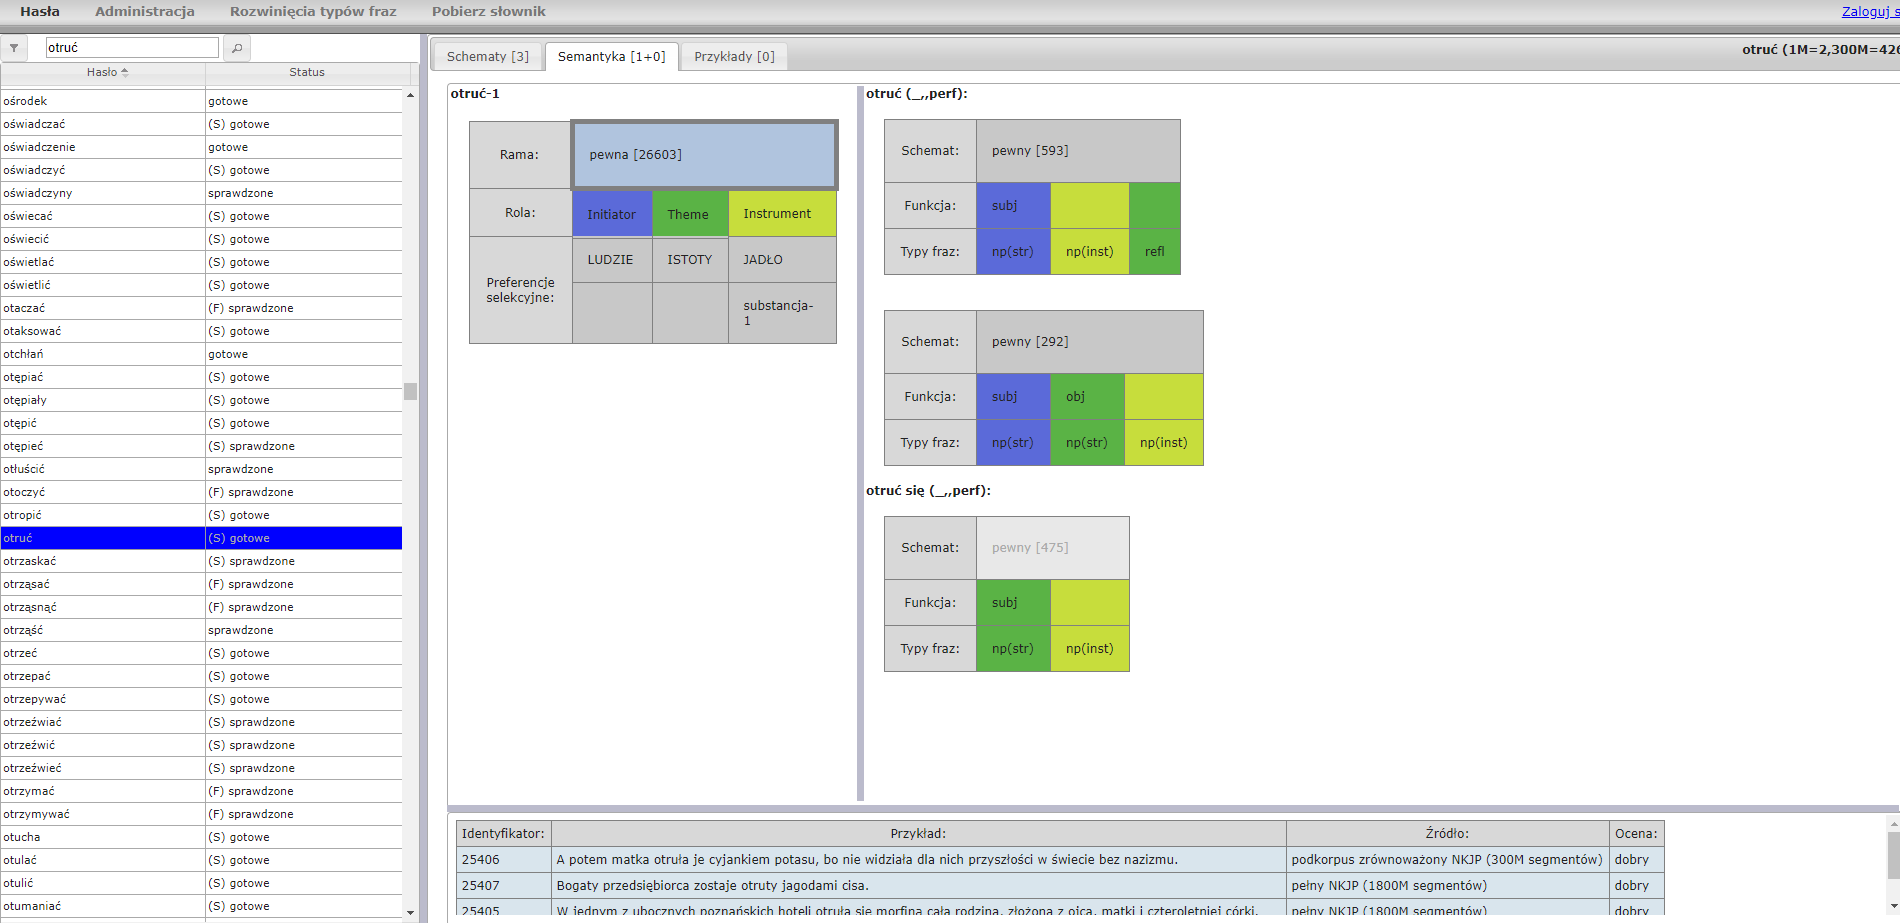
\includegraphics[width=4.7244in,height=3.0181in,width=\textwidth]{grabowski-img001.png}
 
\end{styleStandard}

\begin{styleStandard}
\textit{Figure 1. The verb otruć ‘to poison’ in Walenty (retrieved from: http://walenty.clarin-pl.eu/)}
\end{styleStandard}

\begin{styleStandard}
Although \textit{Walenty} is similar to Pattern Grammar in that it presents syntactic environments of lexical items, it does not allow the researcher to browse through larger lexico-grammatical patterns (e.g. verbs, nouns or adjectives and the words or syntagmatic frames that follow or precede the words) or to classify the slot-fillers in those patterns into specific meaning or functional groups, which is precisely what the Pattern Grammar approach does. For example, the so-called ‘introductory \textit{it}’ pattern followed by a link-verb, adjective and to-infinitive clause (\textbf{\textit{it}}\textbf{ v-link ADJ }\textbf{\textit{to}}\textbf{{}-inf})\footnote{\textrm{The example is available at: https://grammar.collinsdictionary.com/grammar-pattern/it-v-link-adj-to-inf\_1}} reveals a number of meaning groups for adjectives filling in the pattern (Figure 2) as well as specific examples of their use (Figure 3).
\end{styleStandard}

\begin{styleStandard}
  [Warning: Image ignored] % Unhandled or unsupported graphics:
%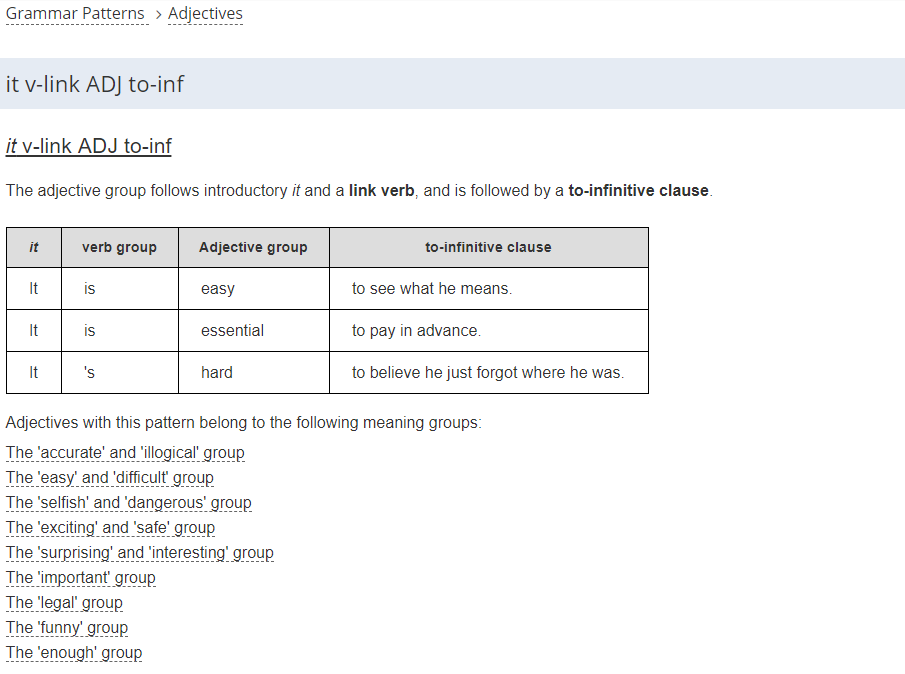
\includegraphics[width=4.7244in,height=2.5929in,width=\textwidth]{grabowski-img002.png}
 
\end{styleStandard}

\begin{styleStandard}
\textit{Figure 2. The pattern ‘it v-link ADJ to-inf’}
\end{styleStandard}

\begin{styleStandard}
  [Warning: Image ignored] % Unhandled or unsupported graphics:
%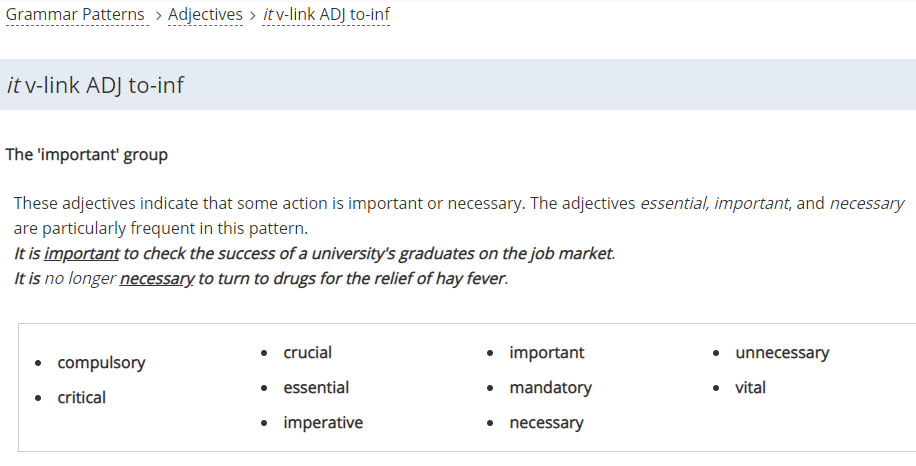
\includegraphics[width=4.7244in,height=2.3575in,width=\textwidth]{grabowski-img003.png}
 
\end{styleStandard}

\begin{styleStandard}
\textit{Figure 3. The pattern ‘it v-link ADJ to-inf’ filled with adjectives conveying the sense of importance.}
\end{styleStandard}

\begin{styleStandard}
As can be seen in Figure 3, the sense of importance (or attitudinal stance) of the following proposition is conveyed by the entire grammar pattern \textbf{\textit{it}}\textbf{ v-link ADJ }\textbf{\textit{to}}\textbf{{}-inf} rather than by individual adjectives filling in the pattern. Consequently, Pattern Grammar offers an inventory of lexico-grammatical constructions which constitute pairings of form with semantic or discoursal function.\footnote{\textrm{In practice, identification of GPs is possible by analyzing concordance lines, which later involves grouping the patterns into notional categories (e.g. topical or functional ones) on the basis of different types of meanings conveyed in contexts. Although individual words can help in determination of those groupings, a qualitative analysis of a wider context of their occurrence is necessary to form appropriate groups and thus identify the patterns (Hunston \& Francis 2000: 162).}} Such a resource describing lexico-grammatical patterns extracted from corpora in a bottom-up fashion has not been developed for the Polish language so far. 
\end{styleStandard}

\begin{styleStandard}
The main goal of this study is therefore to explore whether GPs may be employed as a useful exploratory tool for cross-linguistic studies. In other words, we aim to identify and describe lexico-grammatical patterns that emerge from the English-to-Polish translations – extracted from Paralela corpus (Pęzik 2016) – of a pre-selected English GP performing specific discoursal functions. More precisely, we will focus on one English ‘introductory it’ pattern with \textit{to}{}-clause complementation (\textbf{\textit{it }}\textit{v-link}\textbf{\textit{ ADJ to-inf}}), which will constitute the starting point for our analysis.\footnote{\textrm{Both patterns were studied by Groom (2005) in terms of their variability across different academic registers.}} However, the \textit{tertium comparationis} are the functional categories or discoursal functions (necessity, importance, obviousness etc.) contingent on individual words filling in the patterns or, in other words, worked out on the basis of intuitive understandings of words in the English GPs. This will allow us to investigate whether we may find corresponding generalizable lexico-grammatical patterns in Polish that perform the same discoursal functions as the English GP under scrutiny. The underlying assumption is that in theory the Polish translations should convey the same information as their English source texts. We will also attempt to verify whether GPs are useful as a discovery tool for detecting translation patterns. We believe that a study like this one may pave the way to a wider application of the Pattern Grammar approach for the description of languages other than English (in this case, Polish) and/or for cross-linguistic comparisons or translation-oriented research, which have not been attempted hitherto. 
\end{styleStandard}

\begin{styleStandard}
The chapter is structured as follows. In Section 2, the research material (i.e. the study corpus), units of analysis and methodology will be described. Next, we describe and discuss the empirical results exemplifying translation patterns emerging from textual realizations of GPs in the sample of English source-texts and their Polish translations. The concluding section discusses the study limitations and offers suggestions on how this research may be developed further in the future.
\end{styleStandard}

\begin{listWWNumxxiileveli}
\item 
\begin{stylelsSectioni}
Methodology
\end{stylelsSectioni}

\begin{listWWNumxxiilevelii}
\item 
\begin{stylelsSectionii}
Research material
\end{stylelsSectionii}
\end{listWWNumxxiilevelii}
\end{listWWNumxxiileveli}
\begin{styleStandard}
For the purposes of the current study, we will use the English-Polish parallel corpus \textit{Paralela} (Pęzik 2016), which is available at: http://paralela.clarin-pl.eu. The parallel corpus under scrutiny includes a little more than 262 million word tokens in 10,877,000 translation segments from various text types and genres, including written, spoken and to-be spoken texts, e.g. legal documents from various European Union institutions (legislation, transcripts of proceedings of the European Parliament etc.), press releases, medical texts, film subtitles, popular science texts, literary classics, transcripts of European Parliament proceedings etc. As a rule, a parallel corpus contains source texts aligned with their translations in the target language. In this study, we will analyze a pre-selected GP (‘\textit{it} v-link ADJ \textit{to}{}-inf’) found in a single genre of English source texts, namely European Parliament proceedings (henceforth EPP), and we will try to align its textual realizations with their Polish equivalents as found in translation segments in the corresponding Polish sub-corpus (with more than 13 million word tokens in almost 700,000 translation segments)\footnote{The transcripts were originally extracted from Europarl corpus (Koehn 2005) and included in Paralela (Pęzik 2016). The debates were recorded on 11-12th and 23rd October 2006, and translated from English into Polish.} Then, we will attempt to quantitatively and qualitatively analyze the target language equivalents and see whether any regular patterns, i.e. lexico-syntactic associations similar to GPs, emerge from the Polish language data.
\end{styleStandard}

\begin{listWWNumxxiileveli}
\item 
\begin{listWWNumxxiilevelii}
\item 
\begin{stylelsSectionii}
Units of analysis
\end{stylelsSectionii}
\end{listWWNumxxiilevelii}
\end{listWWNumxxiileveli}
\begin{styleStandard}
At least in theory, parallel corpora include texts (originals and translations) that express the same meanings and perform the same discoursal functions, which allows one to search for correspondences between linguistic items in source and target texts (Johansson 2007: 9, cited in Marco 2019: 43). As mentioned earlier, in this study we will focus on a pre-selected GP, which means that the lexical items under scrutiny will not be extracted from texts in a bottom-up approach. This is mainly because we do not have access to full texts collected in \textit{Paralela}. Hence, the use of the study corpora will be limited to the analysis of bilingual concordances illustrating particular translation patterns, i.e. frequency and distribution of the Polish equivalents of the English GP, which provide a starting point for our investigation. 
\end{styleStandard}

\begin{styleStandard}
We will capitalize on the results of the study conducted by Groom (2005), who analyzed, among others, two GPs, namely \textbf{\textit{it }}\textbf{v-link}\textbf{\textit{ ADJ that}} and \textbf{\textit{it }}\textbf{v-link}\textbf{\textit{ ADJ to-}}\textbf{inf}. Groom (2005: 259-260) noticed that adjectives which convey the meaning (i.e. sense) that can be generalized as “validity” (e.g. \textit{clear, inconceivable, obvious}) tend to fall into the pattern \textbf{\textit{it }}\textbf{v-link }\textbf{\textit{ADJ that}}\textit{ }while the adjectives conveying the sense of “difficulty” (e.g. \textit{difficult, easy, hard}) tend to fall into the pattern \textbf{\textit{it }}\textbf{v-link}\textbf{\textit{ ADJ to-}}\textbf{inf}\footnote{However, Groom (2005) found that distributions and more fine-grained rhetorical functions of the adjectives in those grammar patterns vary across corpora representing different language varieties.}. Also, it was found that depending on the pattern, one and the same word (e.g. the adjective \textit{possible}) may convey different senses, that is either “difficulty” or “validity” (Groom 2005: 259). In summary, the findings of the study conducted by Groom (2005) provide strong evidence of the relationship between particular sense conveyed by particular words and the structural patterns in which those words tend to occur.
\end{styleStandard}

\begin{styleStandard}
We will search for a single pre-selected pattern using the SlopeQ query syntax implemented in \textit{Paralela} (Pęzik 2016) as well as morphosyntactic tags (e.g. \textit{{\textless}tag=j.*{\textgreater}} stands for adjectives). Thus, the pattern \textbf{\textit{it }}\textbf{v-link}\textbf{\textit{ ADJ to-}}\textbf{inf} will be searched for using the following query:
\end{styleStandard}

\begin{listWWNumxxivleveli}
\item 
\begin{styleListParagraph}
\textit{it {\textless}tag=v.*{\textgreater} {\textless}tag=j.*{\textgreater} to} (34,047 occurrences in Paralela; 3,067 occurrences in EPP).
\end{styleListParagraph}
\end{listWWNumxxivleveli}
\begin{styleStandard}
In view of a high number of occurrences, it is necessary to filter out the results to facilitate the qualitative analysis of concordance lines. To this end, we will apply systematic sampling by recording translation pairs of every 30\textsuperscript{th} concordance. This means that we will ultimately focus on a sample of 100 translation pairs (i.e. bilingual concordances illustrating Polish translations of specific textual realizations of the English GP) extracted from the EPP sub-corpus of \textit{Paralela}.
\end{styleStandard}


\setcounter{listWWNumxxiileveli}{0}
\begin{listWWNumxxiileveli}
\item 

\setcounter{listWWNumxxiilevelii}{0}
\begin{listWWNumxxiilevelii}
\item 
\begin{stylelsSectionii}
Research questions and hypotheses
\end{stylelsSectionii}
\end{listWWNumxxiilevelii}
\end{listWWNumxxiileveli}
\begin{styleStandard}
The main problem addressed in this study concerns whether the corresponding items (translation equivalents) found in target texts can also be described in terms of recurrent lexico-syntactic associations similar to the GP identified in the English source texts. Hence, in this exploratory paper we aim to provide answers to the following research questions:
\end{styleStandard}

\begin{styleStandard}
1) What are the Polish equivalents of the English source-language multi-word items emerging from GPs?
\end{styleStandard}

\begin{styleStandard}
2) Can the Polish equivalents be generalized into a more abstract set of lexico-grammatical patterns similar to GPs?
\end{styleStandard}

\begin{styleStandard}
3) Can the Pattern Grammar approach be used for a description of Polish? 
\end{styleStandard}

\begin{styleStandard}
4) Can GPs be applied as a unit of analysis in cross-linguistic contexts? 
\end{styleStandard}

\begin{listWWNumxxiileveli}
\item 
\begin{listWWNumxxiilevelii}
\item 
\begin{stylelsSectionii}
Research questions and hypotheses
\end{stylelsSectionii}
\end{listWWNumxxiilevelii}
\end{listWWNumxxiileveli}
\begin{styleStandard}
This study will be conducted in a number of stages. First, we will preselect one GP (described earlier) and develop an inventory of their textual realizations in English source-texts, i.e. in the EPP sub-corpus of \textit{Paralela}. Then, we will generalize the results by means of grouping overlapping textual realizations into a list of n-grams performing specific discourse functions. After identification of the Polish equivalent, or translation variant (be it a single-word or a multi-word unit), we will investigate whether the observed patterns of Polish translations can be generalized to a more abstract phraseological, syntagmatic or lexico-grammatical units, similar to GPs.
\end{styleStandard}

\begin{listWWNumxxiileveli}
\item 
\begin{stylelsSectioni}
Preliminary results: grammar patterns in contrast
\end{stylelsSectioni}
\end{listWWNumxxiileveli}
\begin{styleStandard}
In this exploratory study, we used the GP \textbf{\textit{it }}\textbf{v-link}\textbf{\textit{ ADJ to-}}\textbf{inf} as a unit of analysis and a tool for discovering potential translation patterns. All in all, the said GP occurred in the EPP sub-corpus of Paralela (Pęzik 2016) 3,067 times. In order to limit the amount of data for manual analysis of bilingual concordances, we used systematic sampling and selected every 30\textsuperscript{th} concordance, which resulted in the set of 100 English-Polish translation segments to be analyzed. Depending on the adjectives filing in the slot, we used the procedure put forward by Groom (2005) and – by conducting manual analysis of English source-text fragments – we classified the textual variants of the GP found in the sample into semantic/functional categories (discoursal functions) corresponding to the senses conveyed by the adjectives. This way, the linguistic data were classified into the following categories: ‘importance’, ‘validity’, ‘desirability’ and ‘difficulty’.
\end{styleStandard}

\begin{styleStandard}
First, we present the results of the analysis of the textual instantiations of the GP \textbf{\textit{it }}\textbf{v-link}\textbf{\textit{ ADJ to-}}\textbf{inf} as filled with adjectives conveying the sense of ‘difficulty’ in the English-original texts in the EPP sub-corpus (8 occurrences) and its equivalents in the Polish translations.
\end{styleStandard}

\begin{flushleft}
\tablefirsthead{}
\tablehead{}
\tabletail{}
\tablelasttail{}
\begin{supertabular}{|m{1.1045599in}|m{1.1615599in}|m{1.0990599in}|m{1.1184598in}|}
\hline
\textbf{Textual realizations in the English-original} &
\textbf{Discoursal function} &
\textbf{Polish equivalents} &
\textbf{Generalized pattern of Polish translations }\\\hline
\textit{it is }\textbf{\textit{difficult }}\textit{to} (5) &
DIFFICULTY &
\textbf{\textit{trudno}}\textit{ jest} (5) &
ADV v-link v-inf\\\hline
\textit{it is }\textbf{\textit{hard}}\textit{ to} (2) &
DIFFICULTY &
\textbf{\textit{trudno}}\textit{, aby} (1)

\textbf{\textit{trudno}} (1) &
ADV, \textit{aby} 

ADV v-inf\\\hline
\textit{it is }\textbf{\textit{easier}}\textit{ to} (1) &
DIFFICULTY &
\textbf{\textit{łatwiej}} (1)  &
ADV v{}-inf\\\hline
\end{supertabular}
\end{flushleft}
\begin{styleStandard}
\textit{Table 1. Textual realizations of the GP }\textbf{\textit{it v-link ADJ to-inf}}\textit{ in English source-texts and their Polish translations: discoursal function of difficulty}
\end{styleStandard}

\begin{styleStandard}
The findings (Table 1) show that in the sample under scrutiny there are three different instantiations of the English GP ‘\textit{it} v-link ADJ \textit{to}{}-inf’ when filled with adjectives conveying the sense of ‘difficulty’, namely \textit{it is difficult to}, \textit{it is hard to} and \textit{it is easier to}, with the total frequency of 8. Those multi-word items have the following Polish equivalents in Paralela corpus (Pęzik 2016), such as \textit{trudno jest} (used 5 times as an equivalent of \textit{it is difficult to}), \textit{trudno, aby }and\textit{ trudno} (used 1 each as equivalents of \textit{it is hard to}) and \textit{łatwiej} (used once as an equivalent of \textit{it is easier to}). Apart from insights into certain translational choices, it has been possible to reconstruct abstract lexico-grammatical patterns (or syntagmatic frames) based on the Polish equivalents and conveying the sense of difficulty with respect to the following proposition, e.g. ‘ADV v-link v-inf’ (\textit{trudno jest}) or ‘ADV v-inf’, both followed by a verb in infinitive form (\textit{trudno jest udowodnić ‘}it is difficult to prove’\textit{, trudno uwierzyć }‘it is difficult to believe’) or ‘ADV, \textit{aby}’ (\textit{trudno, aby }etc.) followed by a complement clause, e.g.:,
\end{styleStandard}

\begin{styleStandard}
\textbf{\textit{It is hard to}}\textit{ believe when reading it. }
\end{styleStandard}

\begin{styleStandard}
\textbf{\textit{Trudno }}\textit{uwierzyć w te słowa, kiedy się je czyta.} [EVOeRj]
\end{styleStandard}

\begin{styleStandard}
\textit{This is because }\textbf{\textit{it is difficult to}}\textit{ prove that the service rendered was of poor quality. }
\end{styleStandard}

\begin{styleStandard}
\textit{Dzieje się tak dlatego, że }\textbf{\textit{trudno jest}}\textit{ udowodnić, że świadczone usługi były złej jakości.} [qoavWA]
\end{styleStandard}

\begin{styleStandard}
\textit{Simplification of the common agricultural policy is a beautiful idea, and }\textbf{\textit{it is hard to}}\textit{ imagine that someone would oppose it. }
\end{styleStandard}

\begin{styleStandard}
\textit{Uproszczenie wspólnej polityki rolnej to piękna idea i }\textbf{\textit{trudno, aby}}\textit{ ktoś był jej przeciwny.} [ea2Eoq]
\end{styleStandard}

\begin{styleStandard}
As can be seen, the English GP ‘\textit{it} v-link ADJ \textit{to}{}-inf’, when filled by adjectives conveying the sense of ‘difficulty’, corresponds to a set of Polish syntagmatic patterns, such as ‘ADV, \textit{aby + }complement clause’, ‘ADV v-link v-infinitive’ or ‘ADV v-infinitive’.
\end{styleStandard}

\begin{styleStandard}
The following example under scrutiny refers to the GP ‘\textit{it} v-link ADJ \textit{to}{}-inf’ as filled with adjectives (\textit{possible, clear, impossible, true}) conveying the sense of ‘validity’ in the English-source texts (Table 2).
\end{styleStandard}

\begin{flushleft}
\tablefirsthead{}
\tablehead{}
\tabletail{}
\tablelasttail{}
\begin{supertabular}{|m{1.0177599in}|m{0.7538598in}|m{1.4379599in}|m{1.2740599in}|}
\hline
\textbf{Textual realizations in the English-original} &
\textbf{Discoursal function } &
\textbf{Polish equivalents} &
\textbf{Generalized pattern of Polish translations }\\\hline
\textit{(will) it be }\textbf{\textit{possible}}\textit{ to} (1) &
VALIDITY &
\textbf{\textit{możliwe }}\textit{(będzie)} (1) &
ADJ v-link\\\hline
\textit{it is }\textbf{\textit{clear}}\textit{ to (us/me)} (2) &
VALIDITY &
\textit{dla (nas) }\textbf{\textit{jasne}}\textit{ jest, że} (1)

\textit{jest dla (mnie) }\textbf{\textit{jasne}}\textit{, że} (1) &
ADJ v-link,\textit{ że} ‘that’

v-link ADJ, że ‘that’\\\hline
\textit{it is }\textbf{\textit{impossible}}\textit{ to} (1) &
VALIDITY &
\textbf{\textit{niemożliwością}}\textit{ jest} (1) ‘impossibility is’

\textit{nie można} (1) ‘ &
NN v-link

NEGprt + MOD v \\\hline
\textit{it is }\textbf{\textit{possible}}\textit{ to} (4) &
VALIDITY &
\textbf{\textit{możliwe}}\textit{ jest} (2) ‘possible that’

\textit{można} (1) ‘may/can’

\textit{możliwość}\footnotemark{} (1) ‘possibility’ &
ADJ v-link

MODv v-inf

TRANSFORMATION\\\hline
\textit{it is }\textbf{\textit{true}}\textit{ to} (1) say  &
VALIDITY &
\textbf{\textit{prawdą}}\textit{ jest, że} (1) ‘truth is that’ &
NN v-link, \textit{że} ‘that’\\\hline
\end{supertabular}
\end{flushleft}
\footnotetext{\textrm{(EN)}\textrm{\textit{ }}\textrm{\textit{I would like to say that }}\textrm{\textbf{\textit{it is becoming clear}}}\textrm{\textit{ in this discussion that it is possible to have a 'two-speed' Europe. }}\textrm{(PL)}\textrm{\textit{ Chciałbym powiedzieć, że w tej dyskusji }}\textrm{\textbf{\textit{oczywista staje się możliwość}}}\textrm{\textit{ istnienia Europy {\textquotedbl}dwóch szybkości”.}}\textrm{ }\textrm{[Drag45]}}
\begin{styleStandard}
\textit{Table 2. Textual realizations of the GP ‘it v-link ADJ to-inf’ in English source-texts and their Polish translations: discoursal function of validity}
\end{styleStandard}

\begin{styleStandard}
The findings show that there is more variety among Polish lexico-grammatical patterns that convey the sense of ‘validity’ in the Polish translations as compared with the sense of ‘difficulty’. The most frequent one (4 occurrences) is the pattern ‘ADJ v-link’ (with positional variation) and ‘ADJ v-link, \textit{że}’, which is realized with the following Polish equivalents, namely \textit{możliwe} (\textit{będzie}); \textit{możliwe jest;} (…) \textit{jasne jest, że}; \textit{jest }(…) \textit{jasne, że}. Other patterns are centred around nouns (‘NN’, ‘NN v-link’ and ‘NN v-link, \textit{że}’), which include the following words and phrases: \textit{możliwość}, \textit{niemożliwością jest} and \textit{prawdą jest, że} respectively, e.g.:
\end{styleStandard}

\begin{styleStandard}
\textit{I would like to say that it is becoming clear in this discussion that }\textbf{\textit{it is possible to}}\textit{ have a 'two-speed ' Europe. }
\end{styleStandard}

\begin{styleStandard}
\textit{Chciałbym powiedzieć, że w tej dyskusji oczywista staje się }\textbf{\textit{możliwość}}\textit{ istnienia Europy {\textquotedbl}dwóch szybkości}\footnote{\textrm{The phrase }\textrm{\textit{Europa dwóch szybkości}}\textrm{ ‘two-speed Europe’ has not been adopted in the Polish press discourse. Instead, the phrase }\textrm{\textit{Europa dwóch prędkości}}\textrm{ has become commonly used. }}\textit{”.}[Drag45]
\end{styleStandard}

\begin{styleStandard}
There are also two patterns centred on the modal verb \textit{można} ‘can/may’ (‘MODv’, ‘NEG PRT MODv’), namely \textit{można} and \textit{nie można}, followed by the infinitive form of the verb, e.g.:
\end{styleStandard}

\begin{styleStandard}
(…) \textit{but the one thing I have learned is that }\textbf{\textit{it is impossible to}}\textit{ book a ticket on the Eurostar when you are travelling}.
\end{styleStandard}

\begin{styleStandard}
(…) \textit{lecz nauczyłem się jednego, a mianowicie, że }\textbf{\textit{nie można}}\textit{ zarezerwować biletu na pociąg}. [BNzRG4]
\end{styleStandard}

\begin{styleStandard}
A large group of multi-word items in the English originals conveys a sense of ‘importance’ (e.g. \textit{it is important to, it is crucial to, it is essential that}) and there is a high variety among their Polish equivalents, which can be grouped into a number of lexico-grammatical patterns. The most prominent ones include the pattern ‘ADJ v-link’ and ‘ADJ v-link, \textit{aby/by’ }(e.g. \textit{istotne jest}; \textit{ważne jest, aby}; \textit{niezbędne jest; konieczne jest}), with adjectives occasionally modified by adverbs (e.g. \textit{bardzo ważne jest}, \textit{niezwykle istotne jest}). It is particularly noticeable that the pattern ‘ADJ v-link’ is followed by a verbal noun functioning as a direct object, while the pattern ‘ADJ v-link, \textit{aby/}by’ or ‘ADJ, \textit{by}’) is followed by the verb in the infinitive form, e.g.:
\end{styleStandard}

\begin{styleStandard}
\textit{Finally, I would like to stress that }\textbf{\textit{it is important to}}\textit{ have full transparency regarding the founding of the initiative and sources of financial support for the organisers.}
\end{styleStandard}

\begin{styleStandard}
\textit{Wreszcie, pragnę podkreślić, że }\textbf{\textit{ważne jest}}\textit{ zapewnienie pełnej przejrzystości w odniesieniu do finansowania inicjatywy oraz źródeł wsparcia finansowego dla jej organizatorów }[RDwmvo]
\end{styleStandard}

\begin{styleStandard}
\textbf{\textit{It is important to}}\textit{ overcome the current problems that characterise the sector: the lack of competition, the regulatory over-dependence on ratings, and the low reliability of notes. }
\end{styleStandard}

\begin{styleStandard}
\textbf{\textit{Ważne jest, aby}}\textit{ rozwiązać problemy, które obecnie spotyka się w tej branży, a mianowicie przesadne zawierzanie ratingom i małą wiarygodność ocen.} [APaN8r]
\end{styleStandard}

\begin{styleStandard}
Other frequent patterns include ‘MODv v-inf’ (\textit{trzeba, musimy/musi, należy }followed by verbs in the infinitive form) or ‘NN ADJ v-link’ (e.g. \textit{sprawą podstawową jest}; \textit{ważną rzeczą jest/są}) or ‘V ADJ NN’ (e.g. \textit{ma fundamentalne znaczenie}), cf. Table 3 below.
\end{styleStandard}

\begin{flushleft}
\tablefirsthead{}
\tablehead{}
\tabletail{}
\tablelasttail{}
\begin{supertabular}{|m{0.98095983in}|m{0.90525985in}|m{1.7920599in}|m{0.9045598in}|}
\hline
\textbf{Textual realizations in the English-original} &
\textbf{Discoursal function} &
\textbf{Polish equivalents} &
\textbf{Generalized pattern in Polish translations }\\\hline
\textit{it is }\textbf{\textit{important }}\textit{to} (1) &
IMPORTANCE &
\textbf{\textit{ważne}}\textit{ jest, aby} (1) &
ADJ v-link, \textit{aby}\\\hline
\textit{it is }\textbf{\textit{crucial}}\textit{ to} (2) &
IMPORTANCE &
\textbf{\textit{istotne}}\textit{ jest} (1)

\textbf{\textit{kluczowe}}\textit{ znaczenie ma} (1) &
ADJ v-link

ADJ NN V\\\hline
\textit{it is }\textbf{\textit{essential}}\textit{ to} (10) &
IMPORTANCE &
\textbf{\textit{konieczne }}\textit{jest} (2)

\textbf{\textit{kluczowe}}\textit{ znaczenie ma} (2)

\textbf{\textit{niezbędne}}\textit{ jest} (2)

\textit{trzeba} (1)

\textit{ma }\textbf{\textit{istotne znaczenie}}\textit{ }(1)

\textbf{\textit{niezwykle}}\textit{ }\textbf{\textit{istotne}}\textit{ jest} (1)

\textit{należy} (1) &
ADJ v-link

ADJ NN V

ADJ v-link

MODv v-inf

V ADJ NN

(ADV) ADJ v-link

MODv v-inf\\\hline
\textit{it is }\textbf{\textit{fundamental}}\textit{ to} (1) &
IMPORTANCE &
\textit{ma }\textbf{\textit{fundamentalne znaczenie}} (1) &
V ADJ NN\\\hline
\textit{it is }\textbf{\textit{imperative}}\textit{ to} (1)  &
IMPORTANCE &
\textbf{\textit{bardzo ważne}}\textit{ jest} (1) &
(ADV) ADJ v-link\\\hline
\textit{it is }\textbf{\textit{important}}\textit{ to} (24) &
IMPORTANCE &
\textit{należy} (6) 

\textbf{\textit{ważne}}\textit{ jest} (6)

\textit{musimy} (1)

\textit{należy }\textbf{\textit{koniecznie}} (3)

\textbf{\textit{ważne}}\textit{ jest, aby} (2)

\textit{trzeba} (2)

\textbf{\textit{bardzo ważne}}\textit{ jest} (1)

\textbf{\textit{konieczne}}\textit{ jest} (1)

\textbf{\textit{ważną rzeczą}}\textit{ jest/są} (1)

\textbf{\textit{ważne}}\textit{, by} (1)

\textbf{\textit{najważniejsze}}\textit{ jest} (1) &
MODv v-inf

ADJ v-link 

MODv v-inf

MODv ADV v-inf

ADJ v-link, \textit{aby}

MODv v-inf

ADJ v-link

ADJ v-link

ADJ N v-link

ADJ, \textit{by}

ADJ v-link\\\hline
\textit{it is }\textbf{\textit{necessary}}\textit{ to} (15) &
IMPORTANCE &
\textit{należy} (4)

\textbf{\textit{konieczne}}\textit{ jest} (3)

\textit{wymaga}\footnotemark{} (2)

\textit{trzeba} (2)

\textit{trzeba }\textbf{\textit{koniecznie}} (1)

\textit{rzeczą }\textbf{\textit{konieczną }}\textit{jest} (1)

\textit{musi} (1) &
MODv v-inf

ADJ v-link

V

MODv v-inf

MODv ADV v-inf

NN ADJ v-link

MODv v-inf\\\hline
\textit{it seems }\textbf{\textit{fundamental}}\textit{ to} (1) me &
IMPORTANCE &
\textbf{\textit{sprawą podstawową}}\textit{ jest} (1) &
NN ADJ v-link\\\hline
\textit{it was }\textbf{\textit{essential}}\textit{ to} (1) &
IMPORTANCE &
\textit{było (jest) }\textbf{\textit{niezwykle istotne}} (1) &
v-link ADV ADJ \\\hline
\end{supertabular}
\end{flushleft}
\footnotetext{\textrm{(EN) }\textrm{\textit{There is also a need to measure quality of life in societies, because in order to ensure and sustain quality of life, }}\textrm{\textbf{\textit{it is necessary to}}}\textrm{\textit{ take into account important, consensual factors such as health, education, culture, employment, housing, environmental conditions etc.}}\textrm{ }\textrm{(PL) }\textrm{\textit{Istnieje także potrzeba pomiaru jakości życia w społeczeństwach, ponieważ osiągnięcie oraz utrzymanie odpowiedniej jakości życia }}\textrm{\textbf{\textit{wymaga}}}\textrm{\textit{ (‘requires’) uwzględnienia istotnych i jednomyślnie uznanych czynników, takich jak zdrowie, edukacja, kultura, zatrudnienie oraz warunki mieszkaniowe, środowiskowe itp.}}\textrm{ }\textrm{[6nv4bb]}}
\begin{styleStandard}
\textit{Table 3. Textual realizations of the GP ‘it v-link ADJ to-inf’ in English source-texts and their Polish translations: discoursal function of importance}
\end{styleStandard}

\begin{styleStandard}
Finally, similar correspondences can be observed in the case of structures conveying the sense of ‘desirability’ in the English originals and their Polish equivalents (Table 4). The most frequent patterns – with positional variation due to free word order – in the Polish translations were found to be ‘ADJ v-link’ (e.g. \textit{konieczne jest, jest niestosowne, nieodpowiedzialne jest, słuszne jest}), ‘ADV v-link’ (e.g. \textit{dobrze jest}), ‘MODv v-inf’ (e.g. \textit{warto, należy}). The comparison of certain GPs provides interesting insights into cross-linguistic correspondences on the syntactic level. For example, the English pattern ‘\textit{it} v-link ADJ v-inf’ may correspond, among others, to the Polish GP ‘MODv v-inf’, where the position of direct and indirect object with respect to the patterns under scrutiny changes, e.g. 
\end{styleStandard}

\begin{styleStandard}
\textbf{\textit{It is essential to}}\textit{ give people }[Indirect object] \textit{access} [Direct object]\textit{ to healthcare, drinking water and sanitation. }
\end{styleStandard}

\begin{styleStandard}
\textit{Ludziom }[Indirect object] \textbf{\textit{należy}}\textit{ zapewnić dostęp }[Direct object]\footnote{\textrm{Lit. ‘people should be given access’}} \textit{do opieki zdrowotnej, wody pitnej i kanalizacji.} [DrZG0o]
\end{styleStandard}

\begin{styleStandard}
We also identified ready-made formulas corresponding to specific speech acts, (e.g. the polite phrase used after a greeting \textit{Cieszymy się, że jest Pan tu z name }versus \textit{it is nice to have you with us}) or transformations resulting from stylistic changes in the translation as compared to the original. Both fixed formulas and transformations do not fall into GPs that we attempted to identify among the Polish equivalents.
\end{styleStandard}

\begin{flushleft}
\tablefirsthead{}
\tablehead{}
\tabletail{}
\tablelasttail{}
\begin{supertabular}{|m{1.2761599in}|m{1.1018599in}|m{1.3976599in}|m{0.8073598in}|}
\hline
\textbf{Textual realizations in the English-original} &
\textbf{Discoursal function} &
\textbf{Polish equivalents} &
\textbf{Generalized pattern in Polish translations }\\\hline
\textit{it is }\textbf{\textit{necessary}}\textit{ to} (1) &
DESIRABILITY &
\textbf{\textit{konieczne}}\textit{ jest} (1) &
ADJ v-link\\\hline
\textit{it is }\textbf{\textit{advisable}}\textit{ to} (1)  &
DESIRABILITY &
OMISSION\footnotemark{} (1) &
OMISSION\\\hline
\textit{it is }\textbf{\textit{appropriate}}\textit{ to} (1) &
DESIRABILITY &
\textbf{\textit{warto}} (1) ‘it is worth’ &
MODv v-inf\\\hline
\textit{it is }\textbf{\textit{better}}\textit{ to} (1) &
DESIRABILITY &
\textbf{\textit{lepiej}} (1) ‘better’ &
ADV V\\\hline
\textit{it is }\textbf{\textit{fair}}\textit{ to} (1) (\textit{say that…}) &
DESIRABILITY &
\textbf{\textit{uczciwie}}\textbf{ }(1) ‘fairly’ &
TRANSFOR-MATION\footnotemark{}\\\hline
\textit{it is }\textbf{\textit{good}}\textit{ to }(1)\textit{ }know &
DESIRABILITY &
\textbf{\textit{dobrze}}\textit{ jest} (1)  &
ADV v-link\\\hline
\textit{it is }\textbf{\textit{inappropriate}}\textit{ to} (1) &
DESIRABILITY &
\textit{jest }\textbf{\textit{niestosowne}} (1) &
v-link ADJ\\\hline
\textit{it is }\textbf{\textit{irresponsible}}\textit{ to} (1) &
DESIRABILITY &
\textbf{\textit{nieodpowiedzialne}}\textit{ jest} (1) &
ADJ v-link\\\hline
\textit{it is }\textbf{\textit{nice}}\textit{ to} (1) (\textit{have you with us}) &
DESIRABILITY &
\textit{Cieszymy się, że} (1) \textit{jest Pan tu z nami} ‘we are happy to have you here with us’ &
FIXED FORMULA\\\hline
\textit{it is }\textbf{\textit{pointless}}\textit{ to} (1) &
DESIRABILITY &
\textit{nie ma sensu} (1)  &
NEGprt V NN\\\hline
\textit{it is }\textbf{\textit{profitable}}\textit{ to} (1)  &
DESIRABILITY &
\textit{przynosi zysk } &
V NN\\\hline
\textit{it is }\textbf{\textit{right}}\textit{ to} (3)  &
DESIRABILITY &
\textit{należy} (1) 

\textit{jest }\textbf{\textit{słuszne}} (1)

\textbf{\textit{słuszne}}\textit{ jest} (1) &
MODv v-inf

v-link ADJ

ADJ v-link\\\hline
\textit{it is }\textbf{\textit{sensible}}\textit{ to} (1) &
DESIRABILITY &
\textit{(jest) }\textbf{\textit{rozsądne}}\textbf{ }(1) &
v-link ADJ\\\hline
\textit{it is }\textbf{\textit{unacceptable}}\textit{ to} (1)  &
DESIRABILITY &
\textit{nie do przyjęcia jest} (1) &
NEGprt PREP NN v-link\\\hline
\textit{it is }\textbf{\textit{uplifting}}\textit{ to }(1) &
DESIRABILITY &
\textit{świadomość} (…) \textit{podnosi na duchu} (1) ‘awareness of (…) raises sb’s spirits' &
TRANSFOR-MATION\\\hline
\textit{it is }\textbf{\textit{worthwhile}}\textit{ to} (1) &
DESIRABILITY &
\textbf{\textit{warto}}\textbf{ }(1) &
MOD v v-inf\\\hline
\textit{it was }\textbf{\textit{agreeable}}\textit{ to} (1)  &
DESIRABILITY &
\textit{miło było} (1) ‘(it) was nice to’ &
ADV v-link v-inf\\\hline
\end{supertabular}
\end{flushleft}
\addtocounter{footnote}{-2}
\stepcounter{footnote}\footnotetext{\textrm{(EN) }\textrm{\textit{We shall check what you have said, and you can rest assured that, within the context of measures available to the Council and the work on implementing the Pact on Immigration and Asylum, }}\textrm{\textit{we shall look once more at}}\textrm{\textit{ whether }}\textrm{\textbf{\textit{it is advisable to}}}\textrm{\textit{ }}\textrm{\textit{reinforce this point}}\textrm{\textit{ within the framework of the Schengen area.}}\textrm{ }\textrm{(PL) }\textrm{\textit{Sprawdzimy to, o czym pan mówił, i może pan mieć pewność, że w kontekście środków, jakimi dysponuje Rada, oraz prac nad wdrożeniem paktu o imigracji i azylu, }}\textrm{\textit{ponownie przemyślimy}}\textrm{\textit{ }}\textrm{\textit{kwestię udoskonalenia tego elementu}}\textrm{\textit{ w ramach strefy Schengen.}}\textrm{ [AP01Ae]}}
\stepcounter{footnote}\footnotetext{\textrm{(PL) (…) }\textrm{\textit{będzie uczciwie, jeżeli powiem, że (…)}}\textrm{ [rBwJxM]}\par }
\begin{styleStandard}
\textit{Table 4. Textual realizations of the GP ‘it v-link ADJ to-inf’ in English source-texts and their Polish translations: discoursal function of desirability}
\end{styleStandard}

\begin{listWWNumxxiileveli}
\item 
\begin{stylelsSectioni}
Discussion and conclusions
\end{stylelsSectioni}
\end{listWWNumxxiileveli}
\begin{styleQuote}
The findings of our exploratory study indicate that the Pattern Grammar approach holds unexplored potential for cross-linguistic research, of both text-oriented and system-oriented kinds. The approach showcased in our study used a set of GPs as a starting point to identify recurrent English multi-word items with specific meanings (senses) and discoursal functions, which were then aligned with their Polish equivalents. We obtained further empirical evidence against a widely held misconception about translation whereby one has to translate a given fixed phrase from L1 (English) into a corresponding fixed phrase in L2 (Polish). Using this methodology, we were able to obtain a set of lexico-grammatical frames emerging from the English-to-Polish translation patterns in the corpus under scrutiny (EPP). As well as yielding insights into language in use in English-to-Polish translation in the EPP corpus, our methodology revealed a number of novel and valuable cross-linguistic correspondences between formulaic structures in English and Polish. As our study was based on a specific text type, it remains to be seen to what extent those Polish lexico-grammatical patterns can be generalized to other text types or genres (if we adopt a textual perspective), and to the Polish language system (if we adopt a cross-linguistic systemic perspective). Nevertheless, our preliminary results are certainly encouraging. 
\end{styleQuote}

\begin{styleQuote}
The findings of the current study also show that the Pattern Grammar approach holds unexplored potential not only for cross-linguistic studies, but also for the description of recurrent lexico-syntactic constructions found in other languages, such as Polish. Clearly, such a research agenda needs to be pursued with caution in view of the many typological differences between English and Polish (cf. Fisiak 1978; Willim \& Mańczak-Wohlfeld 1997). In practice, what this means is that a “Polish version” of Pattern Grammar will need to be mindful of formal descriptions of Polish, and that we should expect to find non-formally corresponding grammar patterns that convey the same meanings or discourse functions in English and Polish, as was the case with the English GP ‘\textit{it} v-link ADJ \textit{to}{}-inf’ and the lexico-syntactic patterns that emerged from the Polish translations, rather than exact equivalents for each given English GP. Indeed, we may find that there are one-to-one, one-to-many, many-to-many and many-to-one relationships between GPs conveying the same meaning or discourse function in English and Polish. Since adjective complementation patterns have received considerable attention (e.g. Su \& Hunston 2019), it would be useful for future research to conduct analyses that involve other patterns (e.g. \textit{there} v-link \textit{sth/anything/nothing} ADJ \textit{about/in} NP). Since this study concerns translation, it would be also interesting for future research to examine whether the observed translation patterns are triggered by English (due to interference), and if so then to what extent, or whether they are natural and equally formulaic in native Polish texts. Since this preliminary study is exploratory in nature, no frequency threshold was set to verify when an equivalent is regarded as a pattern; however, setting such a threshold will be essential in the future. 
\end{styleQuote}

\begin{styleQuote}
Finally, Pattern Grammar-based descriptions of Polish may also feed into the future development of more comprehensive lexicographic resources, the so-called ‘dictionaries of constructions’ or ‘constructicons’ which are presently being compiled for several European languages, including German (Boas \& Ziem 2018), Swedish (Lyngfelt et al. 2018b) and Russian (Janda et al. 2018)\textsuperscript{ }\footnote{\textrm{According to Janda et al. (2018: 165), the Russian constructicon prioritizes multi-word constructions. }\ }, to name but a few, and which are designed to model entire languages as inventories of constructions at all levels, i.e. from morpheme to discourse. A promising example of this synergy of approaches is provided by Perek \& Patten (2019), who are currently building an English constructicon by semi-automatically combining GPs (as represented by the COBUILD reference works) with the semantic frames and valency relations found in the FrameNet database. Since constructicons may serve lexicographers, language learners as well as NLP applications, it is postulated that such a resource, which could utilize information already available in valency dictionaries (e.g. \textit{Walenty}), should be also developed in the future for the Polish language\footnote{\textrm{The idea of developing a construction grammar of Polish has also been briefly mentioned recently by Wierzbicka-Piotrowska (2019).}}.
\end{styleQuote}

\begin{stylelsSectionii}
Acknowledgements
\end{stylelsSectionii}

\begin{styleQuote}
This research has been funded by the Polish National Agency for Academic Exchange (NAWA) under the agreement no: PPN/BEK/2018/1/00081/, and conducted during a research stay of Łukasz Grabowski at the University of Birmingham (UK).
\end{styleQuote}

\begin{listWWNumxxiileveli}
\item 
\begin{stylelsSectioni}
References
\end{stylelsSectioni}
\end{listWWNumxxiileveli}
\begin{stylelsAbstract}
\textup{Boas, H. \& Ziem, A. (2018). “Constructing a constructicon for German: Empirical, theoretical, and methodological issues”. In: B. Lyngfelt, L. Borin, K. Ohara and T. Timponi Torrent (Eds), Constructicography: Constructicon development across languages. Amsterdam: John Benjamins, 183-228.}
\end{stylelsAbstract}

\begin{stylelsAbstract}
\textup{Charles, M. (2006). ‘Phraseological patterns in reporting clauses used in citation: A corpus-based study of theses in two disciplines.’ English for Specific Purposes 25: 310–331.}
\end{stylelsAbstract}

\begin{stylelsAbstract}
\textup{Charles, M. (2007). 'Argument or evidence? Disciplinary variation in the use of the Noun that pattern in stance construction.' English for Specific Purposes 26: 203–218.}
\end{stylelsAbstract}

\begin{stylelsAbstract}
\textup{Ellis, N.C., O'Donnell, M.B. \& Römer, U. (2014). ‘Second language processing of verb-argument constructions is sensitive to form, function, frequency, contingency, and prototypicality.’~Linguistic Approaches to Bilingualism~4(4): 405-431.}
\end{stylelsAbstract}

\begin{stylelsAbstract}
\textup{Fisiak, J., Lipińska Grzegorek, M. \& Zabrocki, L. (1978). An introductory English-Polish~contrastive grammar. Warszawa: PWN.}
\end{stylelsAbstract}

\begin{stylelsAbstract}
\textup{Fillmore, Ch. (1982). ‘Frame semantics’. In: The Linguistic Society of Korea (eds), }Linguistics in the Morning Calm\textup{. Seoul: Hanshin, 111-137.}
\end{stylelsAbstract}

\begin{stylelsAbstract}
\textup{Francis, G., Manning, E. \& Hunston, S. (1996). Collins COBUILD grammar patterns 1: Verbs. London: HarperCollins.}
\end{stylelsAbstract}

\begin{stylelsAbstract}
\textup{Francis, G., Manning, E. \& Hunston, S. (1998). Collins COBUILD grammar patterns 2: Nouns and adjectives. London: HarperCollins.}
\end{stylelsAbstract}

\begin{stylelsAbstract}
\textup{Goldberg, A. (2006). Constructions at Work. The Nature of Generalization in Language. Oxford: Oxford University Press.}
\end{stylelsAbstract}

\begin{stylelsAbstract}
\textup{Groom, N. (2005). “Pattern and meaning across genres and disciplines: An exploratory study.” A \ Journal of English for Academic Purposes 4: 257-277.}
\end{stylelsAbstract}

\begin{stylelsAbstract}
\textup{Hanks, P. (2008a). {\textquotedbl}Mapping meaning onto use: a Pattern Dictionary of English Verbs{\textquotedbl}. AACL 2008, Utah.}
\end{stylelsAbstract}

\begin{stylelsAbstract}
\textup{Hanks, P. (2008b). “Lexical Patterns: from Hornby to Hunston and beyond”. Afrilex 2008, Stellenbosch.}
\end{stylelsAbstract}

\begin{stylelsAbstract}
\textup{Hanks, P. (2013). Lexical Analysis: Norms and Exploitations. Cambridge. MIT Press.}
\end{stylelsAbstract}

\begin{stylelsAbstract}
\textup{Herbst, T., Heath, D., Götz, D., \& Roe, I. (2004).~A Valency Dictionary of English.~Berlin/New York: De Gruyter.}
\end{stylelsAbstract}

\begin{stylelsAbstract}
\textup{Hunston, S., Manning, E., Francis, G. (1998). Grammar Patterns II: Nouns and Adjectives. London: Collins Cobuild.}
\end{stylelsAbstract}

\begin{stylelsAbstract}
\textup{Hunston, S. \& Francis, G. (2000). Pattern Grammar: A Corpus-driven Approach to the Lexical Grammar of English. Amsterdam: John Benjamins.}
\end{stylelsAbstract}

\begin{stylelsAbstract}
\textup{Janda, L., Lyashevskaya, O., Nesset, T., Rakhilina, E. \& Tyers, F. (2018). “A constructicon for Russian”. In: B. Lyngfelt, L. Borin, K. Ohara and T. Timponi Torrent (Eds), Constructicography: Constructicon development across languages. Amsterdam: John Benjamins, 165-182.}
\end{stylelsAbstract}

\begin{stylelsAbstract}
\textup{Koehn, P. (2005). “Europarl: A Parallel Corpus for Statistical Machine Translation”. In: Conference Proceedings: the tenth Machine Translation Summit, Phuket, Thailand: AAMT, 79-86.}
\end{stylelsAbstract}

\begin{stylelsAbstract}
\textup{Larsson, T. (2016). “The introductory it pattern: Variability explored in learner and expert writing.~Journal of English for Academic Purposes,~22, 64-79.}
\end{stylelsAbstract}

\begin{stylelsAbstract}
\textup{Lyngfelt, B., Borin, L., Ohara, K. \& Timponi Torrent, T. (Eds) (2018a). Constructicography. Constructicon development across languages. Amsterdam: John Benjamins.}
\end{stylelsAbstract}

\begin{stylelsAbstract}
\textup{Lyngfelt, B., \ Bäckström, L., Borin, L., Ehrlemark, A. \& Rydstedt, R. (2018b). “Constructicography at work”. In: B. Lyngfelt, L. Borin, K. Ohara and T. Timponi Torrent (Eds), Constructicography: Constructicon development across languages. Amsterdam: John Benjamins, 41-106.}
\end{stylelsAbstract}

\begin{stylelsAbstract}
\textup{Mason, O. \& Hunston, S. (2004). ‘The automatic recognition of verb patterns: a feasibility study.’ International Journal of Corpus Linguistics 9: 253-270.}
\end{stylelsAbstract}

\begin{stylelsAbstract}
\textup{Perek, F. \& Patten, A. (2019). “Towards an English Constructicon using patterns and frames”. International Journal of Corpus Linguistics, 24(3): 356-386.}
\end{stylelsAbstract}

\begin{stylelsAbstract}
\textup{Pęzik, P. (2016). “Exploring phraseological equivalence with Paralela”. In: E. Gruszczyńska \& A. Leńko-Szymańska (Eds), Polish-Language Parallel Corpora. Warszawa: Instytut Lingwistyki Stosowanej UW, 67-81.}
\end{stylelsAbstract}

\begin{stylelsAbstract}
\textup{Pontrandolfo, G., \& Goźdź-Roszkowski, S. (2014). ‘Exploring the Local Grammar of Evaluation: The Case of Adjectival Patterns in American and Italian Judicial Discourse’. Research in Language 12(1): 71-91.}
\end{stylelsAbstract}

\begin{stylelsAbstract}
\textup{Przepiórkowski, A., Hajic, J., Hajnicz, E. \& Uresova, Z. (2017a). „Phraseology in two Slavic Valency Dictionaries: Limitations and Perspectives”. International Journal of Lexicography, 30(1), 1-38. [10.1093/ijl/ecv048]}
\end{stylelsAbstract}

\begin{stylelsAbstract}
\textup{Przepiórkowski, A., Hajnicz, E., Andrzejczuk, A., Patejuk, A. \& Woliński, M. (2017b).~„Walenty: gruntowny składniowo-semantyczny słownik walencyjny języka polskiego”.~Język Polski, XCVII(1): 30–47.}
\end{stylelsAbstract}

\begin{stylelsAbstract}
\textup{Römer, U., O'Donnell, M.B., \& Ellis, N.C. (2014). ‘Second language learner knowledge of verb-argument constructions: Effects of language transfer and typology.’~The Modern Language Journal~98(4): 952-975.~}
\end{stylelsAbstract}

\begin{stylelsAbstract}
\textup{Römer, U., O'Donnell, M.B., \& Ellis, N.C. (2015). ‘Using COBUILD grammar patterns for a large-scale analysis of verb-argument constructions: Exploring corpus data and speaker knowledge.’ In N. Groom, M. Charles \& S. John (eds.).~Corpora, Grammar and Discourse: In Honour of Susan Hunston. Amsterdam: John Benjamins, 43-71.}
\end{stylelsAbstract}

\begin{stylelsAbstract}
\textup{Su, H., \& Hunston, S. (2019). ‘Language patterns and attitude revisited Adjective patterns, Attitude and Appraisal’. }Functions of Language\textup{ 26(3): 343-371.}
\end{stylelsAbstract}

\begin{stylelsAbstract}
\textup{Wierzbicka-Piotrowska, E. (2019). “Od synonimii składniowej do polisemii konstrukcyjnej (rozważania metodologiczne na przykładzie analizy polskich konstrukcji wyrażających relację przyczynowo-skutkową)”. In: Book of Abstracts. Polish Cognitive Linguistics Association Conference 2019 (September 26-28, 2019, Białystok), 95-96. Retrieved on 21 Nov 2019 from: }\url{http://ptjk2019.uwb.edu.pl/wp-content/uploads/2019/09/PCLA2019-Book-of-Abstracts.pdf}
\end{stylelsAbstract}

\begin{stylelsAbstract}
\textup{Willim, E. \& Mańczak-Wohlfeld, E. (1997). A contrastive approach to problems with English. Warszawa: PWN.}
\end{stylelsAbstract}

\end{document}
